\documentclass[11pt]{standalone}
\usepackage{amssymb}
\usepackage{amsmath}
\usepackage[no-math]{fontspec}
\usepackage{unicode-math}
\usepackage{libertinus}
\usepackage{pgf,xcolor}
\usepackage{tikz}
\usetikzlibrary{arrows.meta, backgrounds, calc}
\usepackage{pgfplots}
\pgfplotsset{compat=newest}

\definecolor{my_darkgray}{HTML}{484949}
\definecolor{my_lightgray}{HTML}{F3F4F4}
\definecolor{my_darkblue}{HTML}{005A94}
\definecolor{my_lightblue}{HTML}{CCDEE9}
\definecolor{my_yellow}{HTML}{FFEC7F}
\definecolor{my_red}{HTML}{E60000}
\definecolor{my_orange}{HTML}{E87846}

% Concrete values: delta = 0.5 s^{-1}
% t(alpha)       = -ln(alpha) / 0.5 = -2 ln(alpha)
% dt/d(alpha)    = -1 / (0.5 * alpha) = -2 / alpha
% At alpha = 0.5: t = 2 ln 2 ≈ 1.3863 s,  dt/dalpha = -4 s

\begin{document}
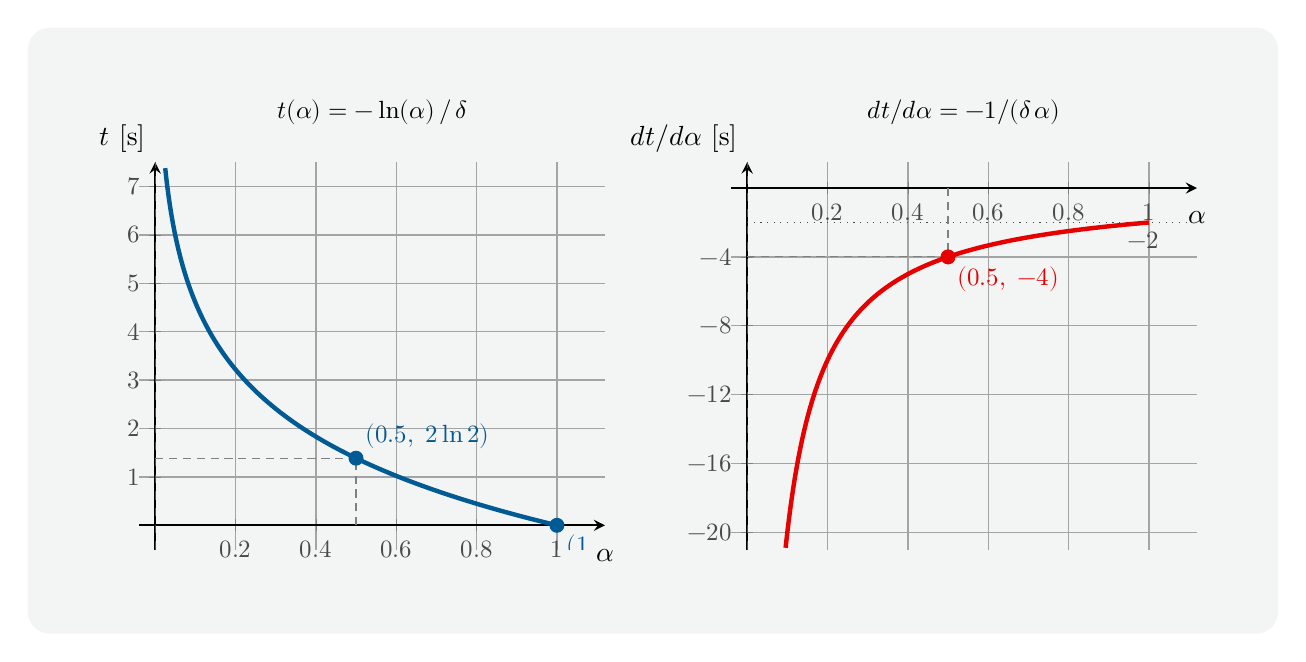
\begin{tikzpicture}[
    show background rectangle,
    background rectangle/.style={fill=my_lightgray, rounded corners=8pt},
    inner frame sep=0.8cm
]

% ── Left plot: t(α) = −2 ln α ───────────────────────────────────────────────
\begin{axis}[
    name=left plot,
    axis lines = center,
    xlabel = {$\alpha$},
    ylabel = {$t~[\text{s}]$},
    xlabel style = {at={(axis cs:1.12,0)}, anchor=north, yshift=-5pt},
    ylabel style = {anchor=south east},
    title = {$t(\alpha)=-\ln(\alpha)\,/\,\delta$},
    title style = {font=\small, text=black, yshift=4pt},
    grid = both,
    grid style = {line width=0.3pt, draw=my_darkgray!30},
    major grid style = {line width=0.5pt, draw=my_darkgray!50},
    % axis equal omitted: α ∈ (0,1], t ∈ [0, ~7 s] – very different scales
    axis line style = {thick},
    xmin = -0.04, xmax = 1.12,
    ymin = -0.5,  ymax = 7.5,
    xtick = {0, 0.2, 0.4, 0.6, 0.8, 1.0},
    ytick = {0,1,2,3,4,5,6,7},
    yticklabel style = {
        /pgf/number format/fixed,
        /pgf/number format/precision=0,
        font=\small,
        text=my_darkgray
    },
    xticklabel style = {
        /pgf/number format/fixed,
        /pgf/number format/precision=1,
        font=\small,
        text=my_darkgray
    },
    width=7.5cm, height=6.5cm,
    clip=true,
]

% Vertical asymptote at α = 0
\addplot[draw=my_darkgray, dashed, thin]
    coordinates {(0,-0.5) (0,7.5)};

% t(α) = -2 ln(α); domain starts away from 0; restrict y as safety net
\addplot[
    draw=my_darkblue,
    samples=500,
    ultra thick,
    domain=0.025:1.0,
    restrict y to domain=0:7.5
]{ -2 * ln(x) };

% Reference point: α = 0.5, t = 2 ln 2 ≈ 1.3863 s
% Drop lines from the point to both axes
\addplot[draw=my_darkgray!70, densely dashed, thin]
    coordinates {(0.5, 0) (0.5, 1.3863)};
\addplot[draw=my_darkgray!70, densely dashed, thin]
    coordinates {(0, 1.3863) (0.5, 1.3863)};

\addplot[
    mark=*,
    mark size=2.5pt,
    only marks,
    draw=my_darkblue,
    fill=my_darkblue
] coordinates {(0.5, 1.3863)};
\node[anchor=south west, font=\small, text=my_darkblue]
    at (axis cs:0.5, 1.3863) {$(0.5,\;2\ln 2)$};

% Mark t(1) = 0: full amplitude → zero settling time
\addplot[
    mark=*,
    mark size=2.5pt,
    only marks,
    draw=my_darkblue,
    fill=my_darkblue
] coordinates {(1.0, 0)};
\node[anchor=north west, font=\small, text=my_darkblue]
    at (axis cs:1.0, 0) {$(1,\;0)$};

\end{axis}

% ── Right plot: dt/dα = −2/α ────────────────────────────────────────────────
% The sensitivity is always negative: a larger target fraction α means
% a shorter (earlier) settling time, hence the negative sign.
% The curve diverges as α → 0⁺ and approaches −2 as α → 1.
\begin{axis}[
    name=right plot,
    at={($(left plot.east)+(1.6cm,0)$)},
    anchor=west,
    axis lines = center,
    xlabel = {$\alpha$},
    ylabel = {$dt/d\alpha~[\text{s}]$},
    xlabel style = {at={(axis cs:1.12,0)}, anchor=north, yshift=-5pt},
    ylabel style = {anchor=south east},
    title = {$dt/d\alpha = -1/(\delta\,\alpha)$},
    title style = {font=\small, text=black, yshift=4pt},
    grid = both,
    grid style = {line width=0.3pt, draw=my_darkgray!30},
    major grid style = {line width=0.5pt, draw=my_darkgray!50},
    % axis equal omitted: sensitivity range −20..0 s vs α range 0..1
    axis line style = {thick},
    xmin = -0.04, xmax = 1.12,
    ymin = -21.0, ymax = 1.5,
    xtick = {0, 0.2, 0.4, 0.6, 0.8, 1.0},
    ytick = {-20,-16,-12,-8,-4,0},
    yticklabel style = {
        /pgf/number format/fixed,
        /pgf/number format/precision=0,
        font=\small,
        text=my_darkgray
    },
    xticklabel style = {
        /pgf/number format/fixed,
        /pgf/number format/precision=1,
        font=\small,
        text=my_darkgray
    },
    width=7.5cm, height=6.5cm,
    clip=true,
]

% Vertical asymptote at α = 0
\addplot[draw=my_darkgray, dashed, thin]
    coordinates {(0,-21.0) (0,1.5)};

% Horizontal asymptote at dt/dα = -2 as α → 1
\addplot[draw=my_darkgray, dotted, thin, domain=0:1.1]{ -2 };
\node[anchor=north east, font=\small, text=my_darkgray]
    at (axis cs:1.05, -2) {$-2$};

% dt/dα = -2/α; restrict y to domain guards against blow-up near α = 0
\addplot[
    draw=my_red,
    samples=500,
    ultra thick,
    domain=0.05:1.0,
    restrict y to domain=-21:0
]{ -2/x };

% Reference point: α = 0.5, dt/dα = -4 s
% Drop lines from the point to both axes
\addplot[draw=my_darkgray!70, densely dashed, thin]
    coordinates {(0.5, 0) (0.5, -4)};
\addplot[draw=my_darkgray!70, densely dashed, thin]
    coordinates {(0, -4) (0.5, -4)};

\addplot[
    mark=*,
    mark size=2.5pt,
    only marks,
    draw=my_red,
    fill=my_red
] coordinates {(0.5, -4)};
\node[anchor=north west, font=\small, text=my_red]
    at (axis cs:0.5, -4) {$(0.5,\;{-4})$};

\end{axis}

\end{tikzpicture}
\end{document}
